\documentclass[ ]{article}
\usepackage[]{amsfonts}
\usepackage[]{amsmath}
\usepackage[ ]{indentfirst}
\usepackage[ ]{graphicx}


\begin{document}

\textbf{1}

	$L(G) = \{ \alpha | \alpha \in (a,b,c)^+$, onde a soma de $a$'s e $c$'s é par se $\alpha$ inicia por $b$, senão $|\alpha|$ é ímpar$\}$
	
	$S ::= a<A>| b<C> | c <A> $ % Inicial
	
	$A ::= a <B> | b<B> | c<B> | \varepsilon$ % inicia por a ou c (|alpha| é ímpar)
	
	$B ::= a <A> | b<A> | c<A>$
	
	$C ::= a<D> | b<C> | c<D> | \varepsilon$ % inicia por b (a+c é ímpar)
	
	$D ::= a<C> | b<D> | c<C>$
	
	
\textbf{2}

	$L(G) = \{\alpha | \alpha \in a^x b^yc^z$ onde $x+z$ é ímpar e $x,y,z>0 \}$
	
	$S::= a <A>$
	
	$A::= a<B> |b<C>$ %x+z ímpar
	
	$B::= a<A>| b<D>$ %x+z par
	
	$C::= b<C> | c<E> $ % x+z ímpar
	
	$D::= b<D> | c<F> $ % x+y par
	
	$E::= c<F>$ % x+y par
	
	$F::= c<E> | \varepsilon$ %x+y ímpar
	
\textbf{3}

	$L(G) = \{ \alpha | \alpha \in (a,b,c)^+$, onde a soma de $a$'s e $c$'s é par se $\alpha$ inicia por $b$, senão $|\alpha|$ é ímpar e $c$ nunca antecede $a\}$
	
	$S::= a<E> | b<A> | c<G>$
	
%inicia por b
	$A::= a<B> | b<A> | c<D> | \varepsilon$ % a+c é par, !c
	
	$B::= a<A> |b<B> | c<C>$ % a+c é ímpar, !c
	
	$C::= b<A>|c<D> | \varepsilon$% a+c é par, c
	
	$D::= b<A>|c<C> $ % a+c é ímpar, c

%inicia por a
	$E::= a<F> | b<F> | c<H> | \varepsilon$ % alpha é ímpar, !c
	
	$F::= a<E> | b<E> | c<G>$ % alpha é par, !c
	
	$G::= b<F> | c<H>| \varepsilon$ % alpha é ímpar, c
	
	$H::= b<E> | c<G>$ %alpha é par, c
	
	\textbf{4}
	
	$L(G) = \{ \alpha | \alpha \in (0$...$9$,$'.'$,$','$,$+$,$-)^+$ onde $\alpha \in \mathbb{R}\}
$

	$digito<= 0 ... 9$
	
	$S'::= +<S> | -<S> | digito<A>$
	
	$S::= digito<A>$
	
	$A::= digito<B> | .<D>| ,<G>| \varepsilon$ % 1 dígito numeral
	
	$B::= digito<C> | .<D> | ,<G> | \varepsilon$ % 2 digitos numeral
	
	$C::=.<D> | ,<G> | \varepsilon$ %3 digitos numeral
	
	% anterior é um ponto (exige a geração de 3 dígitos)
		$D::= digito<E>$
	
		$E::= digito<F>$
	
		$F::=digito<C>$ % obriga a inserção de 1 ponto ou vírgula
	%%%%%%%%%%%%%%%%%
	
	$G::= digito<H>$
	
	$H::= digito<H> | \epsilon$
%	$G::= digito<H> | digito$ %  Essa linha evita a necessidade de criar a regra H pois um símbolo terminal já encerra a sentença
	
	\textbf{Exemplo GLC}
	
	$L(G) =\{ \alpha | \alpha \in a^x c^y$ onde $x>y\}$
	
	$S::= a<S>c | a<A>$
	
	$A::= a<A> | \varepsilon$
	
	$L(G) =\{ \alpha | \alpha \in a^x c^y$ onde $x!=y\}$
	
	$S::= a<S>c | a<A> | <B>c$
	
	$A::= a<A> | \varepsilon$
	
	$B::= <B>c | \varepsilon$
	
	$L(G) =\{ \alpha | \alpha \in a^x b^y c^z$ onde $x!=z$ e $y>0\}$
	
	$S::= a<S>c| a<A> | <B>c$
	
	$A::= a<A> | b<C>$ % quando gerou o b vai para regra C para gerar n quantidade s de b ou encerrar
	
	$B::= <B>c | b<C>$
	
	$C::= b<C> | \varepsilon$
	
	$L(G) =\{ \alpha | \alpha \in a^x b^y c^z$ onde $y=x+z$ e $x,z>0\}$
	% para cada a gerado, obrigatório gerar um b
	% para cada c gerado, obrigatório gerar um b
	
	$S::= <A><B>$
	
	$A::= a<A>b|ab$
	
	$B::=b<B>c|bc$
	
	
	$L(G) =\{ \alpha | \alpha \in (a,b,c)^+$onde o número de $a$'s é igual ao número de $c$'s $\}$ 
	
% não está correta pois a gramática não precisa seguira a ordem a->b->c
%	$S::= a<A>c$
%	
%	$A::= a<A>c |b<B> | \varepsilon$
%	
%	$B::= b<B> | \varepsilon$
	
	$S::= a<> | b<> | c<> | \varepsilon$
	
	$A::=<B><C><B>\textbf{a}<B><C><B>\textbf{c}<C><B> | <B><C><B>\textbf{c}<B><C><B>\textbf{a}<B><C><B> | \varepsilon | <B>$
	
	$B::= b<B> | \varepsilon$
	
	$L(G) = \{ \alpha | \alpha \in (a^{2i+1}b^{i+3} / i>0) \cup (a^{i+4}b^{i+3}/i\geq 0)\}$
	
	$S::= aaa<A>bbbb | aaaa<B>bbb$ % um desvio para cada regra da União
	
	$A::= aa<A>b | \varepsilon$ % contando i com 1 (i>0)
	
	$B::= a<B>b | \varepsilon$ % contando i com 0 (i>=0)
	
	$L(G) = \{ \alpha | \alpha \in ($para, var, = , até, $\{$, $\}$, opl, op, se, então, senão$)^+$ onde $\alpha$ permite estruturas aninhadas de condição e iteração$\}$ %opl operação lógica op operação aritmética %<<<<<<<<<<<<<
	
	$S::= A | B | op$
	
	$A::=$ se opl então {S} $C$
	
	$B::=$ para  $var = var$ até var \{S\}
	
	$C::=$ senão \{S\}  $| \varepsilon$
%	para var opl var { var = var }
%
%	var = var op var
%
%	se var opl var entao var = var senao var = var
%
%	var = var


	
	
	\newpage

%\textbf{4}
%	 Minha tentativa antes da correção do professor
%	$L(G) = \{ \alpha | \alpha \in (0...9, +,-,'.',',')^+$e $d \in \mathbb{R}\}$
%
%	$NUMEROS::= 0 | 1 | 2 | 3 | 4  | 5 | 6 | 7 | 8 | 9 $
%	
%	$POSITIVOS::=  1 | 2 | 3 | 4  | 5 | 6 | 7 | 8 | 9 $
%	
%	$SINAIS ::= + | -$
%	
%	$PONTO ::= .$
%	
%	$VIRGULA ::= ,$
%	
%	$ZERO::= 0$
%	
%	$S::= SINAIS <A> | ZERO<> | POSITIVOS<A>$
%	% Faltou diferenciaro  número de dígitos para procurando ponto quando começa com positivo e quando começa com sinal. Portanto os dois não podem direcionar para A em S.
%	% vou comentar essa resposta para prestar atenção na explicação do professor
%	
%% comecou com sinal
%	$A::= ZERO<B> | POSITIVOS<Q0>|VIRGULA<DECIMAL>$
%	
%	$Q0::= NUMEROS<PP>|PONTO <Q1>| VIRGULA<DECIMAL>$
%	
%	$Q1::= NUMEROS<Q2>$
%
%	$Q2::= NUMEROS<Q3>$	
%
%	$Q3::= NUMEROS<Q4>$
%	
%	$Q4::= PONTO <Q1> | VIRGULA<DECIMAL>$	
%	
%	$PP ::= NUMEROS<PP2>|PONTO<Q1>| VIRGULA<DECIMAL>$
%	
%	$PP2 ::= PONTO<Q1> | VIRGULA<DECIMAL>$
%	$B::= VIRGULA <DECIMAL>$
%	
%	$DECIMAL::= NUMEROS<DECIMAL>$

	\section*{Lista 1 - Gramáticas Regulares}
	
	\textbf{a}
	
	$L(G) = \{x | x \in (a,b)^*$onde o número de $b$'s é par$\}$
	
	$S::= a<B> | b<A> | \varepsilon$
	
	$B::= a<B> | b<A> | \varepsilon$ % b é par
	
	$A::= a<A> | b <B> $ % b é ímpar
	
	\textbf{b}
	
	$L(G) = \{x | x \in (a,b)^*$onde o número de $b$'s é par$\}$
	
	$S::= a<A> | b<B> $ % b é par
	
	$A::= a<A> | b<B>$ % b é par
	
	$B::= a<B>| b<A> | \varepsilon$ % b é ímpar
	
	\textbf{c}
	
	$L(G) = \{ x|x \in (a,b,c)^*$onde ocorra pelo menos dois padrões $'ac'\}$
	
	$S::= a<B> | b<A> | c<A>$
	
	% primeira repetição
	$A::= a<B> | b<A> | c<A>$ % anterior não é a 
	
	$B::= a<B> | b<A> | c<C>$ % anterior é a
	
	% segunda repetição
	$C::= a<D> | b<C> | c<C>$ % anterior não é a
	
	$D::= a<D> | b<C> | c<E>$ % anterior é a
	
	% já cumpriu o requisito
	$E::= a<E> | b<E> | c<E> | \varepsilon$
	
	\textbf{d}
	
	$L(G) = \{ x|x \in (a,b,c)^*$onde ocorra pelo menos um padrão $'abc'\}$
	
	$S::= a<B> | b<A> | c<A>$ 

	$A::= a<B> | b<A> | c<A>$ %anterior não é a
	
	$B::= a<B> | b<C> | c<A>$ %anterior é a
	
	$C::= a<B> | b<A> | c<D>$ % anterior é ab
	
	$D::= a<D> | b<D> | c<D> | \varepsilon$ % pode encerrar
	
	\textbf{e}
	
	$L(G) = \{ x|x \in (0,1)^*$onde o número de $1$'s é múltiplo de $3\}$
	
	$S::= 0<S> | 1<A> | \varepsilon$% K mod 3 = 0	
	
	$A::= 0<A> | 1<B>$ % K mod 3 = 1
	
	$B::= 0<B> | 1<S> $ % K mod 3 = 2
	
	\textbf{f}
	
	$L(G) = \{ x | x \in (a,b,c,d)^+$onde a soma de $a$'s e $c$'s é ímpar se $x$ começa com $a$ ou a soma de $a$'s e $d$'s é par se $x$ começa por $b$; se $x$ inicia por $c$ ou $d$ não existe restrição$\}$
	
	$S::= a<A> | b<C> | c<E> | d<E> $ % inicio
	
	$A::= a<B> | b<A> | c<B> | d<A> | \varepsilon$ % inicia por a & a+c é ímpar
	
	$B::= a<A> | b<B> | c<A> | d<B>$ % inicia por a & a+c é par
	
	$C::= a<D> | b<C> | c<C> | d<D> | \varepsilon$ % inicia por b & a+d é par

	$D::= a<C> | b<D> | c<D> | d<C>$ % inicia por b & a+d é ímpar	
	
	$E::= a<E> | b<E> | c<E> | d<E> | \varepsilon$
	\section*{Lista 2 - Autômatos Finitos}
		\textbf{a}
		
		$S::= 0<S> | 1<S> | 0<A> | 0<C> | 1<B>$
		
		$A::= 0<A> | 0<C> | 0$
		
		$B::= 1<B> | 1$
		
		$C::= 0<C> | 0<A> | 0$
		
		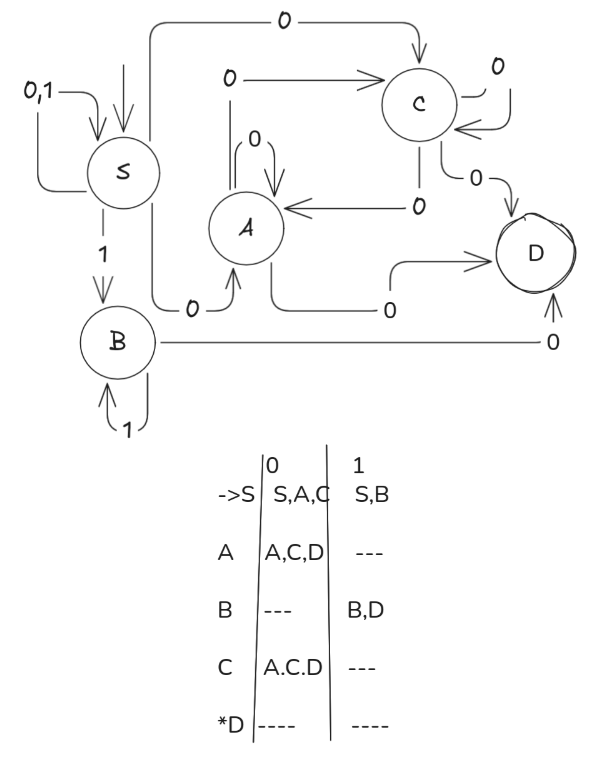
\includegraphics[scale=0.5]{../images/automato-exemplo-1.png}
		
		\textbf{b}
		
		$S::= a<A> | a<C> | b<B> | b<C>$
		
		$A::- a<F> | a$
		
		$B::= b<F> | b$
		
		$C::= a<A> | a<C> | b<B> | b<C>$
		
		$F::= a<F> | b<F> | a | b$
		
		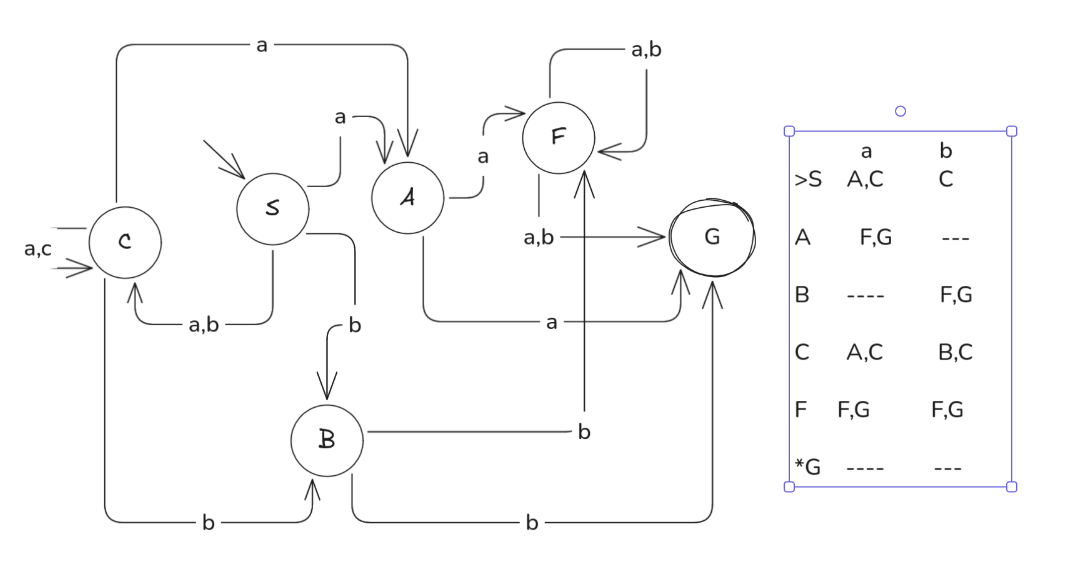
\includegraphics[scale=0.5]{../images/automato-exemplo-2.png}
		
	\section*{Lista de exercícios nova}
		\subsection{4 - autômatos finitos}
		\textbf{d} % Corrigida pelo professor
		
		$S::= 0<B> | 1<A> | 1 | \varepsilon$
		
		$A::= 0<B> | \varepsilon$
		
		$B::= 0<C> | 0 | 1<D>$
		
		$C::= 0<B> | 1<A> | 1$
		
		$D::= 1<C> | 1$
		
		\begin{center}
		AFND\\
		
		\begin{tabular}{ c c c }
  & 0 & 1 \\ 
 $\to$S & B & A,X \\  
 *X & - & - \\
 *A & B & - \\
 B & C, X & D\\
 C& B & A,X\\
 D & - & C, X
		\end{tabular}
		\end{center}
		
		\begin{center}
		AFD\\
		
		\begin{tabular}{ c c c }
   & 0 & 1 \\ 
 $\to$*S & B & [AX] \\  
 B & [CX] & D\\
 *[AX] & B & - \\
 *[CX] & B & [AX]\\
 D & - & [CX]
 		\end{tabular}
		\end{center}
\end{document}
